\documentclass{article}
\title{CSCI 447 Project 2 Design Document}
\author{George Engle, Troy Oster, Dana Parker, Henry Soule}
\usepackage{hanging}
\usepackage{graphicx}
\begin{document}
\maketitle
\section{Introduction}
\quad \quad For this assignment, we are required to assess the performance of five different algorithms on six different data sets. The five algorithms used are $k$-nearest neighbors, edited $k$-nearest neighbors, condensed $k$-nearest neighbors, $k$-means clustering, and $k$-medoids clustering.  The essential purpose of the latter four algorithms is to produce a reduced data set with which to run k-nearest neighbors. We have found literature suggesting improved accuracy among nearest neighbor algorithms that employ data reduction [1][2].  Based on this, we have hypothesized that the average accuracy of $k$-nearest neighbors across all six data sets without reduction will be worse than the average accuracy across the six data sets once reduction has been performed via edited k-nearest neighbors, condensed k-nearest neighbors, k-means clustering, and k-medoids clustering.
%Possible TODO: add in description of loss functions we are using to define 'accuracy'.

\section{Class Descriptions}

\subsection*{Path\_Manager}
\quad \quad This class handles pathing through the project’s databases.This way it is easy to reconfigure or setup for a new database or file type at a moment’s notice.

\subsection*{Database}
\quad \quad  Our database class acts as an instantiable object for holding relevant information from a selected database (project data files).

\subsection*{Process\_Data}
\quad \quad Makes use of the Path\_Manager to target a specified database, then loads in the relevant information from that database, then loads in the relevant information from that database’s directory into a database object which can then be manipulated as we please. \\ \\
-This class also contains functionality for identifying and correcting missing values from a database via bootstrapping statistic. \\ \\
-It also contains functionality for randomly shuffling data in a given database by specific attribute and percentage to modify.

\subsection*{KNN: TODO: INCLUDE CLASS DESCRIPTION HERE?}

\subsection*{Components TODO: REFACTOR INTO OTHER FORMAT!}
\quad \quad Our design has 5 primary components. $database.py$ is a wrapper class that will handle all functionality of each data set. Each instance of the database class will store the processed data of one our six data sets, the the index of the class attribute of its respective database. $knn.py$ will store our implementations of $k$-nearest neighbors, edited $k$-nearest neighbors, and condensed $k$-nearest neighbors. $kcluster.py$ will store the implementation of both clustering algorithms--$k$-means and $k$-medoids clustering. $validation.py$ will perform our 10-fold cross-validation and our loss functions. $main.py$ will perform the execution of our program. 

\section{Design Decisions}

\subsection*{Missing Data handling}
\quad \quad When a dataset is identified to have missing data, we identify the sets of data with missing attributes, and move them from the database’s stored data matrix into a separate list of the sets of data with missing attributes. Once the missing data has been identified, we substitute values for the missing attribute via bootstrapping random values from the set of data that does not contain any missing attributes as our means of imputation. \\ \\
\quad \quad We opted not to simply remove data, even if under a certain threshold, as we assumed it would be more likely to impact our results than including data that would be discredited if incorrect by other present data. 
Additionally, we don’t have a static value to symbolize a missing value, but rather one must be specified for a given dataset in the database directory’s .attr file. This approach allows missing values to be considered a category of their own if necessary.

\subsection*{Identifying Categorical vs Discrete (continuous) data}
\quad \quad In order to determine how we should process data, we have decided to use our method from assignment 1 for identifying categorical vs discrete data types to automatically handle which algorithms will be available/valid to use on a given data set.

\subsection*{Nearest Neighbors distance function}
\quad \quad We decided on Euclidean distance as our means of determining nearest neighbors, as manhattan distance didn’t seem to make much sense seeing as it isn’t direct. 

\section{Plan}
\quad \quad To test our hypothesis, we need to compute the average performance of $k$-nearest neighbors across all six of our data sets, and the average performance of each of the other four algorithms across all six data sets. Our program will first perform $k$-nearest neighbors on all six our data sets, performing 10-fold cross-validation for each data set. As we perform our 10-fold cross-validation for $k$-nearest neighbors on each data set, we will compute the average loss function (0-1 Loss for classification data, Mean Squared Error for regression) for the current data set. We will then compute the average overall loss function across all six data sets once we have completed our 10-fold cross-validation for each data set. \\ \\
\quad \quad We will then perform 10-fold cross-validation using the four other algorithms. Each of these algorithms produces a reduced data set with which to work. Thus, we will implement each of these algorithms to output the reduced data set. For each of the reduced data sets produced by each of the four algorithms, we will perform 10-fold cross-validation.

\section{Algorithm Design}

\section{Experimental Design}

\quad \quad In order to test our implementations of the algorithms, we will use classification and regression datasets as indicated in Figure A below. 

\begin{center}
    \makebox[\textwidth]{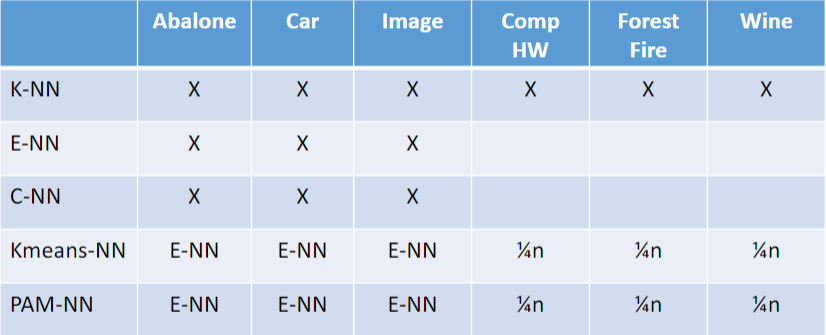
\includegraphics[width=4.75in]{chart.PNG}}
    \caption{Figure A: Project 2 Clarification chart}
\end{center}

\quad For each test, we will use ten-fold cross validation with the equal width binning approach for setting up the training and testing bins from the given dataset.

\subsection*{Handling Tuning}

\quad \quad We will be following the rule of thumb to use the square root of the number of training samples as the initial value for the amount of neighbors (K) used for the nearest neighbors algorithms. From here, however we want to see if we can improve our ability to more accurately represent the model by increasing and decreasing the value of K and checking if it is a better fit.

It is worth noting however, that this method is susceptible to the hill climbing problem, however working our way around that with more iterations would likely result in a drastic increase in the amount of time it takes to find the supposed ‘optimal’ K value, so we may not end up with a perfect solution as we will likely forgo this additional step.

\subsection*{Evaluation}

\quad \quad In order to properly evaluate our implementations, we will split up our evaluation methods for regression and classification based problems into separate functions. This is necessary seeing as classification doesn't involve real values, whereas the regression ones do, hence the innate disconnect and reasoning for identifying and evaluating them separately.

For evaluating regression problems, we need a way of comparing our methods predicted continuous value to the actual continuous value. But we also need this method of measuring our prediction accuracy to be robust with regards to outliers.

So we use Mean Absolute Error (MAE), which measures the sum of the absolute differences between our predicted continuous values and the actual continuous values, and then averages the value by the amount of values compared. ($MAE = \frac{1}{n} \sum_{i=1}^n | y_i - \hat{y}_i|$) As a bonus, it averages the absolute difference is important to note, as it makes MAE resistant to outliers by weighting the individual differences equally. The closer MAE is to 0, the better our predicted line of best fit.

As for evaluating how well our classification predicting implementation performs, we need a way of comparing our predicted classifications and the actual classifications. But this time we don’t really care about outliers, so we use the Mean Squared Error as it tells us how far off our prediction distribution is from the actual distribution (The smaller the MSE, the better our ability to accurately predict the correct classification), and accuracy as metrics for algorithm evaluation. We use accuracy in addition because Mean Squared Error on its own can possibly be 0 on its own which would lead to incorrect classifications.



\subsection*{UML Diagram}
\begin{center}
    \makebox[\textwidth]{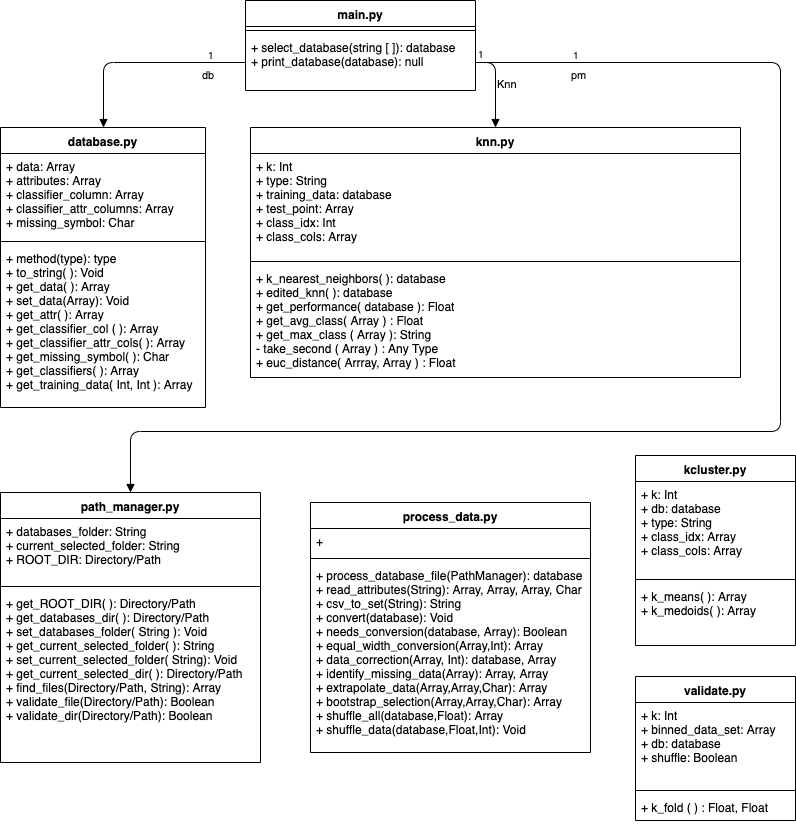
\includegraphics[width=4.75in]{uml}}
\end{center}

\section{Works Cited}
\begin{hangparas}{.25in}{1}
[1] Wagner, T. "Convergence of the Edited Nearest Neighbor (Corresp.)." IEEE Transactions on Information Theory, vol. 19, no. 5, 1973, pp. 696?697., doi:10.1109/tit.1973.1055059.

[2] Nitin Bhatia, V. "Survey of Nearest Neighbor Techniques.: International Journal of Computer Science and Information Security, vol. 8, no. 2. 2010.
\end{hangparas}

\end{document}